\section{RxJS: Reactive Extensions For JavaScript}

Rx ist eine Library, die für zahlreiche Programmiersprachen zur Verfügung gestellt wird. Diese finden sowohl in der Frontend als auch in der Backend-Implementierung Anwendung. In dieser Arbeit wird der Fokus auf RxJS geworfen. Diese Library ist eine Erweiterung speziell für Javascript/Typescript. RxJS erlaubt es mit Hilfe von Observable-Sequenzen Event-basierte Programme zu erstellen. Dabei wird dieser Ansatz auch als \textbf{reactive Programming} definiert. Neben der Kernfunktionalität von Observables werden auch Subjects und Schedulers geboten. Sollte man von reactive Programming noch nichts gehört haben, dann wird die größte Herausforderung sein \glqq{}reactive\grqq{} zu denken.

\subsection{Reactive Programming}
Im Kern ist reactive Programming ein Programmierparadigma. Im \textbf{reaktiven Manifest}, zu finden unter

\begin{center}
\url{https://www.reactivemanifesto.org/de},
\end{center}

\noindent
wird bereits beschrieben, dass Reactive Programming als Programmierung mit asynchronen, unveränderlichen Streams von Events bezeichnet wird. Laut der offiziellen Dokumentation richtet sich ReactiveX nach dem Beobachter-Muster (engl. Observer-Pattern). Das Observer-Pattern ist ein Entwurfsmuster, in der Änderungen eines Objektes (Subjects genannt) an einer Liste abhängiger Strukturen weitergereicht wird. Diese abhängige Strukturen (Observers) werden bei jeder Zustandsveränderung informiert. Eine Veränderung eines Objekts kann hierbei gleichgesetzt werden mit einem neuen Wert innerhalb eines Datenflusses. Als Beispiel für eine reaktive Anwendung kann Excel genommen werden. Ändert man einen Wert in einer Zelle, ändert sich auch der Wert in der Summenzelle. Die Zelle, deren Wert geändert wurde, löst ein Event aus, den die Summen-Zelle empfängt. Daraufhin findet eine Neuberechnung statt.\cite{reactive-programming-beispiel} Datenflüsse können aus verschiedensten Operationen entstehen wie z.B. Klick-Events, Variablen, Cache etc. Als Observer kann man sich in diesem Datenfluss einhängen und entsprechend reagieren.\cite{rx-intro} Rx bietet eine enorme Menge an Funktionen diese Datenflüsse zu bearbeiten/manipulieren (siehe Sektion Operatoren). Diese Operatoren komplett abzudecken wird in dieser Arbeit unmöglich sein, jedoch wird nach dem behandeln dieses Kapitels ein gewisses Grundverständnis für neue Operatoren entstehen und wie diese in Folge anzuwenden sind. Die grundlegenden Konzepte, um asynchrone Events in RxJS zu steuern, sind:

\begin{description}
    \item Observable: Repräsentiert die Idee einer abrufbaren Sammlung, in der zukünftige Werte oder Events gelagert sind.
    \item Subscription: Repräsentiert das Aufrufen eines Observable.
    \item Observer: Ein Objekt, dass eine Sammlung von Callbacks enthält, um die aus dem Observable gelieferten Werte, abzurufen.
    \item Operators: Funktionen, die das Verhalten von Observable-Streams beeinflussen.
    \item Subjects: Eventgeneratoren, die Events an zuhörende Observer zurückgibt. Im Gegensatz zu Observables, sind Subjects standardmäßig multicasting fähig.
    \item Schedulers: Steuerungsmechanismen die bestimmen, wann eine Subscription startet und wann Werte aus dem Stream an die Observer übermittelt werden.
\end{description}


\subsection{Observables}

Observables sind eine träge Sammlung von multiplen Werten. Sie füllen den fehlenden Platz in der unten stehenden Tabelle:

\begin{center}
    \begin{tabular}{| l | l | l |}
    \hline
    & \textbf{Einzelne-} & \textbf{Multiple Werte} \\ \hline
    \textbf{Pull/synchron} & Funktionen & Iterables (Arrays, Strings, ...) \\ \hline
    \textbf{Push/asynchron} & Promises & Observables  \\ \hline
    \end{tabular}
\end{center}

\noindent
Das Push- und Pull-Prinzip beschreibt dabei wie ein Datenproduzent mit dem Datenverarbeiter kommuniziert. In \textbf{Pull-Systemen} bestimmt der Verarbeiter, wann die Daten vom Ersteller angenommen werden. Der Ersteller selbst weiß nicht, wann die Daten angefragt werden. Jede Javascript Funktion unterliegt einem Pull-System. Die Funktion ist ein Verarbeiter von Daten und diese kann im Code jederzeit abgerufen werden.\\

\noindent
Das \textbf{Push-Prinzip} wird im nächsten Beispiel deutlich. Vor dem Ausführen des Beispiels muss ../rxjs/introduction.ts als Eingangsdatei definiert werden.

\begin{figure}[H]
\begin{lstlisting}[basicstyle=\small]
const alias: Observable<number> = RxJS.Observable.create((observer) => {
    observer.next(1);
    observer.next(2);
    observer.next(3);
    setTimeout(() => {
        observer.next(4);
        observer.complete();
    }, 1000);
});

console.log('Before subscribe');
alias.subscribe(next: x => console.log('Value: ' + x));
console.log('After subscribe');
\end{lstlisting}
\end{figure}

\noindent
Das Observable-Objekt repräsentiert eine Kollektion die Werte zu seinen Beobachtern liefert. In diesem Beispiel wird ein Observable erstellt, dass sofort (synchron) die Werte 1, 2 und 3 produziert, sobald die Subscription gestartet wird. Der vierte Wert wird asynchron übermittelt und das Observable daraufhin geschlossen. Die Konsole gibt die Werte in folgender Reihenfolge aus:

\begin{figure}[H]
\begin{center}
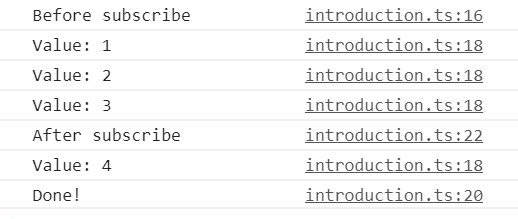
\includegraphics{observable-create-console}
\end{center}
\caption{Observable können sich sich sowohl synchron als auch asynchron verhalten.}
\end{figure}

\noindent
In Push-Systemen steuert der Datenproduzent, wann die Daten an die Datenverarbeiter übermittelt werden. Der Verarbeiter weiß hingegen nicht, wann die Daten ankommen. Promises sind ein typisches Beispiel für Push-Systeme. Ein Promise (Produzent) übermittelt einen eingetroffenen Wert an angeschlossene Callbacks (Verarbeiter). Ungleich wie mit Funktionen bestimmen Promises, wann die Werte an die Callbacks weitergereicht wird. Observables zählen zu einem neuen Push-System in Javascript. Im Gegensatz zu Promises emittieren Observables multiple Werte in Form von Streams. Zur Unterscheidung:

\begin{description}
\item Eine Funktion ist eine träge ausführende Operation, die beim Abruf ein Wert synchron zurückgibt.
\item Ein Promise ist eine Operation die einen eventuell eintreffenden oder nicht-eintreffenden Wert zurückgibt.
\item Ein Observable ist eine träge ausführende Operation, dass synchron oder asynchron keine oder potenziell unendlich viele Werte ab dem Zeitpunkt des Aufrufs zurückgibt.
\end{description}

\noindent
Hierbei stellt sich die Frage, was bedeutet träge? Träge Funktionen, im englischen auch als \textit{lazy Functions} bezeichnet, sind Funktionen die erst bei ihrem Aufruf Werte produzieren.\cite{lazy-functions}

\begin{figure}[H]
\begin{lstlisting}[basicstyle=\small]
function foo() {
    console.log('Hello');
    return 42;
}

const x = foo();
console.log(x);

const bar = RxJS.Observable.create((observer) => {
    console.log('Hello');
    observer.next(42);
});

bar.subscribe((x) => console.log(x));
\end{lstlisting}
\end{figure}

\begin{figure}[H]
\begin{center}
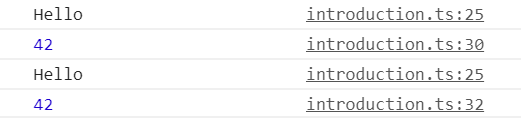
\includegraphics{observable-lazy-console}
\end{center}
\caption{Der Output bleibt immer derselbe.}
\end{figure}

\noindent
Das liegt daran, da sowohl Funktionen als auch Observables träge sind. Die Operationen innerhalb beider Typen findet erst beim Aufruf statt. Mit anderen Worten: Das starten einer Subscription ist analog zum Aufruf einer Funktion. Entgegen der Annahme, dass Observables ausschließlich asynchron operieren, können diese ebenfalls synchron Werte ausgeben (siehe Abb. 22). Der Hauptpunkt in dem Observables sich von Funktionen unterscheiden ist, dass Observables mehrere Werte (mit der Zeit) emittieren können. Innerhalb einer Funktion ist es nicht Möglich zwei return Ausdrücke einzubauen, die zusammen ausgegeben werden.

\subsubsection{Anatomie eines Observable}
Observables werden entweder mit einer der statischen Methoden, mit einer Observable Instanz oder mit der Hilfe eines Observable-Operators \textbf{erstellt}. Der Datenfluss wird an die Observer mit der subscribe() Methode \textbf{überreicht}. Letzteres kann die Exekution der Datenübertragung \textbf{abgesetzt} werden.

\begin{figure}[H]
\begin{lstlisting}[basicstyle=\small]
const randomNumber = new Observable<number>(observer => {
    observer.next(Math.random());
    observer.complete()
});
\end{lstlisting}
\caption{Instantiierung eines Observables, als Parameter wird ein Callback angenommen.}
\end{figure}

\noindent
Die statische Methode Observable.create() ist ein alias ist zum Konstruktoraufruf. Da Observables kein, ein oder unendlich viele Werte ausstoßen können, gibt es Einschränkungen wie Werte an die Observer verteilt werden. Diese Einschränkungen richten sich nach dem sog. \textit{Observable Contract}. Zum Beispiel ist es nicht möglich nachdem Auftreten eines Fehlers oder Fertigstellung eines Observables noch weiter Werte auszugeben:

\begin{figure}[H]
\begin{lstlisting}[basicstyle=\small]
const observable = new Observable<number>(observer => {
  observer.next(1);
  observer.complete();
  observer.next(2);
});
\end{lstlisting}
\caption{Der zweite Wert wird niemals ausgeliefert.}
\end{figure}

\noindent
Um Fehler an die Observer mitzuteilen, ist es üblich die Werte innerhalb eines try-catch Blocks zu verarbeiten:

\begin{figure}[H]
\begin{lstlisting}[basicstyle=\small]
const observable = new Observable<number>(observer => {
  try {
    observer.next(1);
    observer.complete();
  } catch (e) {
    observer.error(e);
  }
});
\end{lstlisting}
\caption{Fehler werden mit der error Funktion gefangen und an die Observer übermittelt.}
\end{figure}

\noindent
Beim erstellen eines Observable, muss sich vor Augen geführt werden, wie die Daten an die Observer überreicht werden sollen. Wenn ein Observable aufgerufen wird, bekommt der Observer einen eigenständigen Datenfluss vom Datenproduzenten zugesprochen. Das hat zur Folge, dass mehrere Observer sich der gleichen Observable-Quelle anschließen und dennoch unterschiedliche Werte bekommen können.

\begin{figure}[H]
\begin{lstlisting}[basicstyle=\small]
const randomNumber = new Observable<number>(observer => {
    observer.next(Math.random());
});

randomNumber.subscribe(value =>
    console.log('1st subscription emits: ', value));
randomNumber.subscribe(value =>
    console.log('2nd subscription emits: ', value));
\end{lstlisting}
\end{figure}

\begin{figure}[H]
\begin{center}
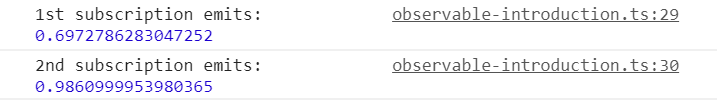
\includegraphics[width=12cm]{unicasting-observables}
\end{center}
\end{figure}

\noindent
Das Ergebnis sind zwei verschiedene Werte, bei zwei Subscriptions - an einem Observable. Diese Eigenschaft wird als \textbf{unicasting} bezeichnet. Das ist nur Möglich, da die Funktion random() erst dann aufgerufen wird, wenn die Datenübertragung gestartet wird. Somit hat jede Subscription eine eigene Ausführung des Datenproduzenten. Es gibt nun mehrere Möglichkeiten, wie sich Observer den gleichen Datenfluss mit der gleichen Quelle teilen. Eine Möglichkeit wäre, den Datenproduzent außerhalb des Observable auszulagern. 

\begin{figure}[H]
\begin{lstlisting}[basicstyle=\small]
const dataProducer: number = Math.random();
const randomNumber = new Observable<number>(observer => {
    observer.next(dataProducer);
});

...
\end{lstlisting}
\end{figure}

\noindent
Eine elegantere Variante, wäre ein Operator anzuwenden, der den zuletzt eingetretenen Wert an die verschiedenen Observer teilt:

\begin{figure}[H]
\begin{lstlisting}[basicstyle=\small]
const multicast = randomNumber.pipe(shareReplay());

multicast.subscribe(value =>
    console.log('1st subscription emits: ', value));
multicast.subscribe(value =>
    console.log('2nd subscription emits: ', value));
\end{lstlisting}
\end{figure}

\noindent
Wie im obigen Beispiel zu sehen ist, werden Operatoren mit der pipe() Methode aus der Observable Klasse angeschlossen. Nun können multiple Subscriptions die gleiche Sequenz von Daten empfangen, da shareReplay() dafür sorgt, dass der Datenproduzent nur einmal aufgerufen werden kann und weitere Subscriptions sich diesen Datenproduzenten teilen. Diese Eigenschaft wird auch als \textbf{multicasting} bezeichnet. Das Ergebnis sieht wie folgt aus:

\begin{figure}[H]
\begin{center}
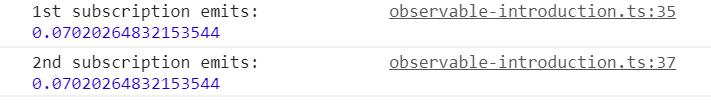
\includegraphics[width=12cm]{multicasting-observables}
\end{center}
\end{figure}

\noindent
Wenn Werte eines Streams erst beim Aufruf einer Subscription entstehen, handelt es sich hierbei um \textbf{cold Observables}.\cite{hot-vs-cold} Dies ist in jedem der oben angeführten Beispielen der Fall. Um auf die oben angeführte These zurückzukommen, dass Observables erst mit der subscribe() Methode Werte ausgeben, war dies zwar zum Einstieg in die Thematik hilfreich, aber nur die halbe Wahrheit. Observables können Werte ausstoßen, unabhängig davon ob eine Subscription stattfindet oder nicht. Hierbei handelt es sich um ein \textbf{hot Observable}. Um einen besseren Einblick zu bekommen, wird ein Observable erstellt, dass unendlich viele Werte ausstößt.

\begin{figure}[H]
\begin{lstlisting}[basicstyle=\small]
const infinite = RxJS.interval(1000).pipe(publish());
infinite.connect();

setTimeout(() =>
    infinite.subscribe(v => console.log('1st subscriber:', v)), 2000);
setTimeout(() =>
    infinite.subscribe(v => console.log('2nd subscriber: ', v)), 3000);
\end{lstlisting}
\caption{Interval gehört zu den Creation Operatoren}
\end{figure}

\noindent
Die statische Methode interval() erstellt ein Observable, dass aufsteigend Nummern innerhalb eines festgelegten Intervalls ausgibt. Der Startindex ist 0. Der publish() Operator sorgt dafür, dass das Observable in einem \textbf{connectable Observable} umgewandelt wird. Das heißt es werden erst Werte innerhalb der Sequenz emittiert, sobald die entsprechende connect() Methode am Observable aufgerufen wird. Alle dazugehörigen Observers bekommen, ab dem Zeitpunkt der Subscription die Werte der Quelle überreicht.\\

\begin{figure}[H]
\begin{center}
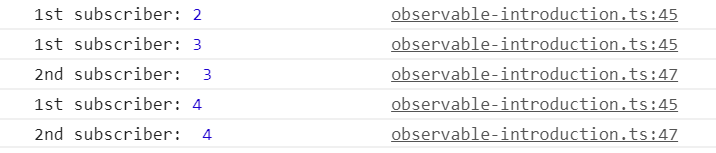
\includegraphics[width=12cm]{hot-observable}
\end{center}
\end{figure}

\noindent
Es vom Observable ab, wann die Sequenz von Werten emittiert werden. Ein hot Observable könnte Werte ausstoßen, sobald es erstellt wird. Und deshalb könnten Observer, die sich später am Observable-Stream einhängen, Werte zwischenzeitlich verpassen. Wenn der gleiche Datenproduzent über verschiedene Subscriptions genutzt wird, ist dies ebenfalls ein Indikator dafür, dass es sich um ein hot Observable handelt. Ein cold Observable dagegen wartet mit dem emittieren der Werte, bis eine Subscription eines Observers stattgefunden hat. Dieser Observer empfängt dementsprechend die gesamten Werte der Sequenz. In manchen Versionen von Rx gibt es auch die Bezeichnung connectable Observable. In solchen Fällen werden erst dann Werte emittiert, wenn die dazugehörige connect() Methode aufgerufen wurde, unabhängig davon ob eine Subscription an dem Observable stattfindet oder nicht.\cite{hot-vs-cold-part-2}

\subsection{Subscription}

Da Observables potenziell unendlich viele Werte an dessen Observer ausgeben können, ist es üblich, dass ab dem Zeitpunkt, an denen die Werte nicht mehr gebraucht werden, die Übertragung gestoppt wird. Insbesondere bei cold Observables ist die Übertragung der Werte exklusiv. Um keine Rechenleistung oder Speicherressourcen zu verschwenden, können daher Subscriptions aufgegeben werden.

\begin{figure}[H]
\begin{lstlisting}[basicstyle=\small]
const subscriber: Subscription = multicast.subscribe(value => console.log(value));

firstSubscriber.unsubscribe();
\end{lstlisting}
\end{figure}

\noindent
Wenn also die subscribe() Methode aufgerufen wird, bekommt der Observer eine eigenständige Observable Exekution. Dieser Aufruf gibt dabei ein Subscription Objekt zurück. Mit diesem Objekt ist es daraufhin möglich \textbf{unsubscribe()} aufzurufen, um die Exekution zu stoppen. Es sollte dabei beachtet werden, dass nur die Übertragung an die jeweilige Subscription gestoppt wird.

\subsection{Observer}

Ein Observer ist der Verarbeiter der übertragenen Werte eines Observables. Das Observer Objekt hat für jede Art der Übertragung eine eigene Funktion:

\begin{figure}[H]
\begin{lstlisting}[basicstyle=\small]
const observer: Observer<number> = {
    next: x => console.log('Got a next value: ' + x),
    error: err => console.error('Got an error: ' + err),
    complete: () => console.log('Got a complete notification')
};
\end{lstlisting}
\end{figure}

\noindent
Eines der Funktionen wird aufgerufen, wenn:

\begin{description}
\item next: ein Wert ausgegeben wird,
\item error: ein Fehler auftritt,
\item complete: sich der Stream schließt.
\end{description}

\noindent
Daraufhin kann das Observer Objekt als Argument in die Subscription übergeben werden:

\begin{figure}[H]
\begin{lstlisting}[basicstyle=\small]
observable.subscribe(observer);
\end{lstlisting}
\end{figure}

\noindent
Es ist jedoch auch Möglich die Funktionen, direkt in subscribe() als Argument anzugeben. Es wird dann intern ein Observer Objekt erstellt mit der ersten Funktion als den next Callback. Wenn alle drei Callbacks als Argument eingegeben werden, sieht das so aus:

\begin{figure}[H]
\begin{lstlisting}[basicstyle=\small]
observable.subscribe(
  x => console.log('Got a next value: ' + x),
  err => console.error('Got an error: ' + err),
  () => console.log('Got a complete notification')
);
\end{lstlisting}
\end{figure}

\subsection{Operatoren}
Wenn es um Operatoren geht, sind diese die wahre Stärke der Observables. Operatoren manipulieren das Stream-Verhalten oder beeinflussen die Werte innerhalb eines Streams. Deshalb ist es mit ihnen möglich komplexen asynchronen Code, leicht und deklarativ zusammenzustellen.\\

\noindent
Operatoren sind Methoden eines Observable Objekts. Wenn ein Operator an einem Observable angewendet wird, wird eine neue Observable Instanz mit einem neuen Datenfluss erstellt. Der ursprüngliche Datenfluss wird nicht verändert. Das liegt daran, dass Observables an sich unveränderlich sind. Bei Anwendung wird somit das aktuelle Observable als Input genommen und ein neues Observable als Output generiert. Deshalb wird bei einer Subscription des Output Observable auch eine des Input Observables stattfinden. Im folgenden Beispiel wird ein selbstkreiertes Observable erstellt, dass alle numerischen Werte mit 10 multipliziert:

\begin{figure}[H]
\begin{lstlisting}[basicstyle=\small]
function multiplyByTen(input): Observable<number> {
   return RxJS.Observable.create(function subscribe(obs) {
        input.subscribe(val => obs.next(val * 10),
            err => obs.error(err),
            () => obs.complete()
        );
    });
}

const observable = from([1, 2, 3, 4]);
const output = multiplyByTen(observable);
output.subscribe(res => console.log(res));
\end{lstlisting}
\end{figure}

\noindent
Die Subscription des Outputs verursacht implizit eine des Inputs. Dieses Verhalten wird \textbf{Operatoren Subscription Kette} genannt. In einem Marble-Diagramm abgebildet, welches standardmäßig für die visuelle Darstellung von Operatoren in Rx genutzt wird, sieht der Fluss wie folgt aus:

\begin{figure}[H]
\centering
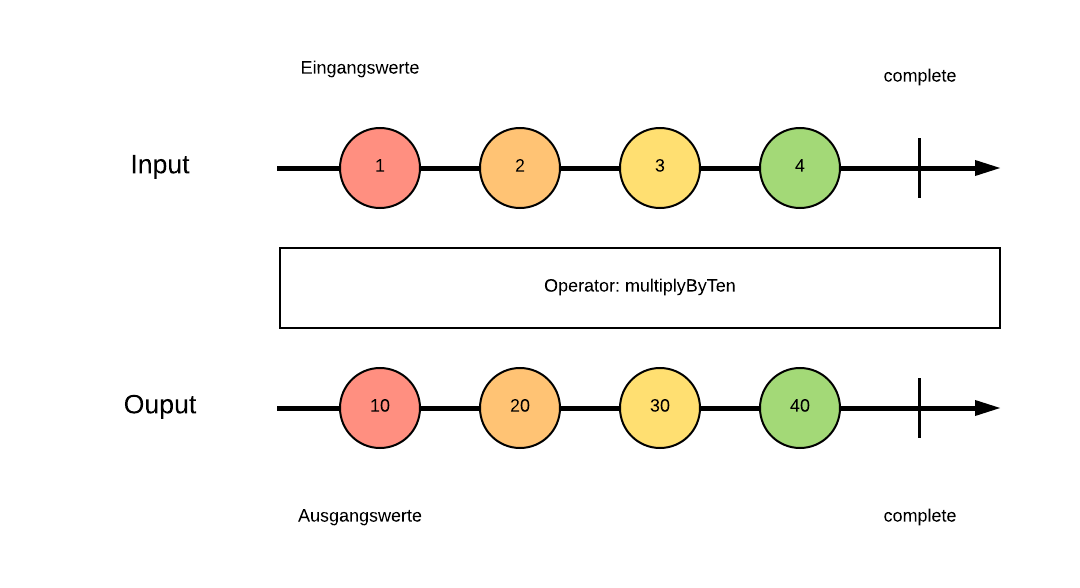
\includegraphics[width=12cm]{multiplybyten-fluss}
\end{figure}

\subsubsection{Instanz Operatoren und statische Operatoren}
Ein Instanz Operator, ist eine Methode die nur innerhalb einer Observable Instanz aufrufbar ist. Wenn die obige Methode eine offizielle Observable Methode sein würde, würde ihre Implementierung wie folgt aussehen:

\begin{figure}[H]
\begin{lstlisting}[basicstyle=\small]
RxJS.Observable.prototype.multiplyByTen = function() {
    const input = this;
    return RxJS.Observable.create(observer => input.subscribe(val => observer.next(val * 10),
        err => observer.error(err),
        () => observer.complete()
        )
    );
};
\end{lstlisting}
\end{figure}

\noindent
Instanz Operatoren sind Funktionen die den this Ausdruck als Referenz der Input Observable nutzen. Das Input Observable wird nicht mehr als Callback genutzt, sondern als Funktionsaufruf eines Observable Objekts.

\begin{figure}[H]
\begin{lstlisting}[basicstyle=\small]
const observable = RxJS.from([1, 2, 3, 4]).multiplyByTen();
observable.subscribe(result => console.log(result));
\end{lstlisting}
\end{figure}

\noindent
Ein statischer Operator hingegen ist eine Funktion, die direkt an die Observable-Klasse angehängt wird. Für gewöhnlich werden dabei Observable auf Anhieb erstellt. Die typischsten statischen Operatoren sind die creation Operatoren. Anstatt ein Input-Observable als Argument anzunehmen, wird ein nicht-Observable Objekt als Argument übergeben und somit ein neues Observable erstellt. Als Beispiel kann dabei die Funktion interval genommen werden, die in Abbildung. 23 genutzt wurde. Sie nimmt einen numerischen Wert an und generiert ein neues Observable als Output.\\

\noindent
Im Ausnahmefall gibt es auch Kombinationsoperatoren, die als statische Methoden fungieren, wie z.B: merge(), combineLatest(), concat(), etc. Da hierbei multiple Observables als Input übergeben werden.

\begin{figure}[H]
\begin{lstlisting}[basicstyle=\small]
const observable1 = RxJS.interval(1000);
const observable2 = RxJS.interval(400);

const merged = merge(observable1, observable2);
merged.subscribe(res => console.log(res));
\end{lstlisting}
\end{figure}

\noindent
Das Ergebnis ist ein Kanal aus Streams, in dem beide Quellen in unterschiedlichen Intervallen ihre Werte ausschütten.

\subsubsection{Kategorien von Operatoren}

Es gibt Operatoren für verschiedene Anwendungsfälle und können kategorisiert werden in: Kreation, Transformierung, Kombination, Multicasting und Fehlerbehandlung. Wie ursprünglich bereits erwähnt werden Operatoren mit der pipe() Methode an einem Observable angeschlossen. Da ein Teil der Kreations- und Transformationsoperatoren bereits abgehandelt wurden, wird mit den Kombinationsoperatoren fortgefahren.\\

\noindent
Um komplexe for Schleifen zu umgehen, bietet Javascript nativ die Möglichkeit mit Callback Funktionen Arrays weiterzuverarbeiten.

\begin{figure}[H]
\begin{lstlisting}[basicstyle=\small]
const source = ['1', '2', '5', 'foo', '13', '17', 'bar'];

console.log(source);

const result = source
    .map(val => parseInt(val, 10))
    .filter(num => !isNaN(num))
    .reduce((previous: number, current: number) => previous + current);
\end{lstlisting}
\end{figure}

\noindent
In diesem Fall werden alle Werte in Zahlen umgewandelt und herausgefiltert. Letzteres wird die Summe gebildet. Observables bieten mit Operatoren die gleiche Funktionalität:

\begin{figure}[H]
\begin{lstlisting}[basicstyle=\small]
const result$ = from(source).pipe(
    map(val => parseInt(val, 10)),
    filter(num => !isNaN(num)),
    reduce((previous: number, current: number) => previous + current));

result$.subscribe(res => console.log(res));
\end{lstlisting}
\caption{Mit dem Kreationsoperator from wird jedes Iterable oder \textit{Promiselike} Okjekt in einem Observable umgewandelt.}
\end{figure}

\noindent
In der asynchronen Prozessverarbeitung ist ein häufiger Anwendungsfall asynchrone Operationen voneinander abhängig auszuführen. Wie im Kapitel Callbacks, Promises und Async await bereits gegenübergestellt, kann dieser Anwendungsfall auch mit Observables durchgeführt werden. Im folgenden werden Operatoren vorgestellt die multiple Datenströme in verschiedensten Ausführungen verarbeiten.

\begin{figure}[H]
\begin{lstlisting}[basicstyle=\small]
const observable1 = new Observable(obs => {
    setTimeout(() => {
        obs.next({id: '1', name: 'Marco'});
        obs.complete();
    }, 2000);
});

const observable2 = new Observable(obs => {
    setTimeout(() => {
        obs.next({age: 25, gender: 'male'});
        obs.complete();
    }, 1000);
});
\end{lstlisting}
\end{figure}

\noindent
\textbf{Concat} ist ein statischer Operator der als Argument mehrere Observables annimmt. Dabei werden die übergeben Argumente in einem Output Observable zusammengefasst und sequentiell ausgeführt. Mit anderen Worten: Concat führt eine Subscription des ersten Observable aus und die Werte entstehend aus der Exekution werden emittiert. Nach der Fertigstellung des Observable findet die nächste Subscription des zweiten übergegebenen Arguments statt. Dieser Vorgang wiederholt sich bis die Argumente ausgelaufen sind. Wenn ein Observable nicht fertiggestellt wird, wird concat niemals zur nächsten Subscription voranschreiten.\\

\noindent
Ein üblicher Anwendungsfall ist auch das Zusammenführen Ergebnissen aus  zwei verschiedenen Datenströmen.











\subsection{Subjects}

Ein RxJS Subject ist eine spezialisierte Form von Observables. Hierbei sind die Datenströme von vornherein multicastingfähig. Dabei kennzeichnet ein Subject zwei Merkmale:

\begin{description}
\item Jedes Subject ist auch ein Observable.
\item Jedes Subject ist auch ein Observer.
\end{description}

\noindent
Da man bei Subjects eine Subscription starten kann, bekommen die angeschlossenen Observer die übertragenen Werte. Aus der Sicht des Observers, ist nicht klar ob die Observable Exekution einem Observable oder eines Subjects entstammt. Wie bei einem typischen Verhalten eines Hot Observables, wird kein neuer Datenstrom an den Aufrufer der subscribe() Methode übertragen. Vielmehr wird der neue Observer in einer Liste von Observers registriert.\\

\noindent
Andererseits ist ein Subject ein Objekt, welches die Methoden next(v), error(e) und complete() enthält. Um einen neuen Wert an die zuhörenden Observer zu emittieren, muss nur next() mit dem jeweiligen Wert aufgerufen werden, um den Wert an die registrierten Observer zu verteilen.

\begin{figure}[H]
\begin{lstlisting}[basicstyle=\small]
const subject = new RxJS.Subject();

subject.subscribe(v1 => console.log('ObserverA: ', v1);
subject.subscribe(v2 => console.log('ObserverB: ', v2);

subject.next(1);
subject.next(2);
\end{lstlisting}
\end{figure}

\noindent
In diesem Beispiel wurde ein Subject mit jeweils zwei angeschlossenen Subscriptions erstellt. Dabei wird das Subject mit Werten\glqq gefüttert\grqq. Da ein Subject auch ein Observer sein kann, ist es auch Möglich diesen als Argument einer subscribe() Methode einzusetzen:

\begin{figure}[H]
\begin{lstlisting}[basicstyle=\small]
const subject = new RxJS.Subject();

subject.subscribe(v1 => console.log('ObserverA: ', v1);
subject.subscribe(v2 => console.log('ObserverB: ', v2);

const observable = RxJS.Observable.from([1, 2, 3]);
observable.subscribe(subject);
\end{lstlisting}
\end{figure}

\noindent
Mit diesem Beispiel wurde ein typisches Unicast Observable in ein multicastingfähiges konvertiert. Dies ist ein weiteres Beispiel einer Umwandlung eines cold- in ein hot Observable. Ohne den Datenproduzent außerhalb des Observables zu lagern, sind Subjects die einzige Möglichkeit eine Observable Exekution an mehrere Observer zu verteilen. Mit der ursprünglichen Konvertieren in Abb. 22 wurde mit dem shareReplay() Operator eine Funktion genutzt, die intern mit Subjects arbeitet.\\

\noindent
Es weitere Arten von Subjects, die in Folge gegenübergestellt werden: \textbf{BehaviourSubject}, \textbf{ReplaySubject}, \textbf{AsyncSubject}.

\subsection{Schedulers}

